%!TEX root = ../thesis.tex
%*******************************************************************************
%****************************** Second Chapter *********************************
%*******************************************************************************

\chapter[MC Method]{A Monte Carlo simulation for phonon transport within silicon structures
at nanoscales with heat generation}

\graphicspath{{Chapter2/}}

%\section*{MC Work Abstract}
\setlength{\epigraphwidth}{0.6\textwidth}
\epigraph{“Anyone who wants to analyze the properties of matter in a real problem
might want to start by writing down the fundamental equations and then
try to solve them mathematically. Although there are people who try to
use such an approach, these people are the failures in this field. . . "}
{\textit{Richard Feynman, sugar coating it.}}


\textit{In nanostructures whose characteristic lengths are comparable to the phonon mean free path(MFP), the ballistic-diffusive heat conduction leads to the size effect\cite{hua0}, which means the relationship between the heat flux and the temperature becomes complicated.In this work, an effective Monte Carlo(MC) method on the basis of using a model of phonon scattering process is employed to simulate the ballistic-diffusive heat conduction in silicon nanofilms, which is based on the methods proposed by Hua's work to study the effective thermal conductivity of nanostructures with internal heat source in one dimension\cite{hua0,hua1}.To get a clear vision of the temperature distribution of the chip, I first calculated the phonon transport in a two-dimension silicon nanofilm with internal heat source. The simulation agrees with the the diffusive approximation(Kn<<1), and it clearly shows the size effect in two dimensions.}                
 
%%%%%%%%%%%%%%%%%%%%%%%%%%%%%%%%%%%%%%%%%%%%%%%%%%%%%

\section[Introduction]{A brief introduction}
As the rapid development of microelectronics, an in-depth understanding of nanoscale thermal transport is quite necessary\cite{Dames,hua2}. On one hand,the typical size of the electronic devices have been decreasing at a dramatical speed, just using the example of diode, which is the key component of chips. As is reported in October, 2016, $MoS_2$ transistors with 1-nanometer
gate lengths has been made out\cite{Desai}. On the other hand, the integration of single chip has been doubling per 18 months since the 1950s, causing the heat flux density arrives at as high as $10^5W/cm^2$, which makes it even harder for the cooling of the chips and electronics. Additionally, when the size of silicon decreases to micro even nano scale, the well-known law of heat transfer, namely Fourier's Law fails. The reliability of electronics, however, is sensitive to the temperature fluctuations. When the temperature reaches 70-80 $^\circ$C, the reliability will decrease 5\% if temperature becomes 1 $^\circ$C higher\cite{Flik}. Consequently, great efforts have been devoted to study the phonon transport phenomenon in micro/nano structures, especially the ballistic-diffusive heat conduction in silicon in recent years.\\
\indent Speaking of the heat transport in dielectric material, the heat transport is predominant by phonons which are quanta of crystal vibrational energy\cite{Statisticalmechanics,Ziman}.In bulk materials, phonons usually undergo several scatterings during the transport and the control law is the Fourier's law, $q=-k\nabla T$, where q denotes the heat flux , T denotes the temperature and k is the material constant of heat transfer. While in nanostructures, the characteristic lengths are compatible to the phonon mean free path(MFP), whose physical meaning is the mean distance a phonon can go before scattering occurs, causing some phonons will not undergo scattering before arriving at the boundary, which we call the ballistic transport. Actually, when the size reaches the nano scale, the effect of the boundary becomes quite important and cannot be omitted, and that is the reason why the governing rule and physical picture of nanostructures are so different from in bulk materials. In summary, the heat transport in nanostructures violates the classical rule, and we call the new process the ballistic-diffusive heat conduction.\\
The key point to solve the ballistic-diffusive conduction problem is to solve the famous equation proposed by Boltzmann\cite{Bolt}:
\begin{equation} 
\frac{\partial f}{\partial t} + v_g \nabla f = \frac{f_0 - f}{\tau} + \dot{S}_{\Omega} \label{con:Boltz}
\end{equation}
In which $v_g$ is the group velocity of phonon, f is the phonon distribution function, $f_0$ is the equilibrium distribution function(since phonons are boses, the Bose-Einstein distribution\cite{chandler}),$\tau$ is the relaxation time and $\dot{S}_{\Omega}$ the phonon source per solid angle\cite{hua3}, or more clearly, the internal heat source. What we should notice is that the effect of boundary is not directly included in this equation but its effect will be considered when we impose the boundary conditions when solving that equation.\\
\indent The temperature profile, which is an important point in this problem, is the focus of my work. Studies to gain the better picture of the temperature profile in silicon with internal heat source have been conducted both theoretically\cite{Lu,Amon} and experimentally\cite{Li,hsiao2013observation,Jo}. It has been found that in the ballistic-diffusive regime, if we still get an effective k(which is quite different from the k in bulk material, we just divide the heat flux by temperature gradient, namely, $k_{eff}=q/\nabla T$), significantly reduces as compared to the bulk material. One direct result is the on the condition of the same heat flux, the nano material will get a higher temperature rise compared to the temperature gradient predicted with the bulk material model, which is an urgent issue in electronic cooling.\\ \indent Although these both aspects have made great progress these years, the underling mechanism of the size effect is ambiguous and the general model with concrete physical base to predict the size effect and related other things is still lacking. So several simulation methods and techniques have been developed to help solve the problem.\\
\indent Three types of methods have been adopted to help simulate the phonon ballistic transport using Boltzmann transport equation(BTE): molecular dynamics(MD)\cite{MD},Lattice-Boltzmann method(LBM)\cite{LB} and Monte Carlo(MC)\cite{KL}. Compared with the MC method, MD method is limited in the size for its amount of calculation
and LBM is not suitable for simulation of complicated boundaries. MC method, which is a quite universal method in computational physics, has gained great success in solving many models in quantum and statistical mechanics\cite{Lan}. In our problem, we trace a great number of phonons(usually greater than $10^6$ and also depends on the size of the problem), derive the distribution function through statistics and then get the thermal properties of the material. In a nutshell, MC method actually give a discrete solution to the BTE and thus is more powerful when it comes to the effect of scattering and different boundary conditions.\\
%My highlight
\indent Our work aims at getting the temperature profile of the actual electronic chips, and based on that we can consider some methods to do the optimization. Considering most optimization of chips till now are actually conducted in macro scale, the attempt to do that work in nano scale can help better understand and finally solve the cooling problem.

%%%%%%%%%%%%%%%%%%%%%%%%%%%%%%%%%%%%%%%%%%%%%%%%%%%%%%%%

\section{Methods}
\subsection{Monte Carlo simulation details}
\subsubsection{The gray approximation}
For simplification, we choose the gray approximation in the MC simulation, which has been proved effective and acceptable in past work\cite{hua0,hua1}. The gray media approximation assumes that the phonon properties are frequency-independent, that's to say, the dispersion relationship of phonon is easiest and the $p$ just equals a constant. On operation, we can first get the dispersion relationship of phonon in silicon by quantum mechanics or doing experiments and then find out the frequency interval of which phonons carry the most of the energy to get the typical frequency we choose in MC simulation. Hence, we finally focus on the phonons traveling with one single velocity and we can study the scattering using one average MFP(These point is quite important for us to get the simplified BTE, namely Equation (\ref{con:Boltz})).\\
\indent It is well-accepted to choose the phonon MFP of bulk material, $l_a$, to do the MC simulation. $l_a$, can be calculated using the method of the kinetic theory.
\begin{equation} \label{eq2}
l_a=\frac{2 \lambda_{b}}{C_v v_g}
\end{equation}
where $\lambda_{b}$ is the thermal conductivity of bulk silicon, $C_V$ is the heat capacity whilst keeping the volume constant, $v_g$ is the average group velocity.
For silicon at room temperature, we list the main data in the following chart\cite{Super}.\\

\begin{table}[!hbp]
\centering
\begin{tabular}{|c|c|}
\hline $\lambda_{b}$  &150 W/(m k)\\
\hline $C_v$ & 1.63 $\times 10^6J/(m^3$ k) \\
\hline $v_g$&6400 m/s\\
\hline    
\end{tabular}\\
\caption{Silicon}
\end{table}

But if we explore the dispersion model of phonon in silicon more detailed, we will find the phonons in silicon can be divided into two types of phonons: acoustic phonons and optical phonons. If we only consider the acoustic phonons that carry most of the energy(that is acceptable in room temperature or we only need to consider the optical phonons at ultralow temperature), we get a new value of MFP, 260nm\cite{Super}. Actually, when we consider that new dispersion model, we need to change the corresponding $C_V$ and $v_g$,finally we choose the value at 43.7 nm\cite{hua1,hua2,hua3}.\\
\subsubsection{Relationship between energy and temperature}
We use the MC method to trace the phonons in the nanofilm and we can get the distribution, but we need to know the relationship between the distribution and the temperature to get the temperature profile.
Similar to the photon, the phonon intensity emitting from a black boundary has the form of what is famous as Stephen-Boltzmann rule\cite{HT}(The similarity also lies in the two quasi-particles both being Boses)
\begin{equation} \label{eq3}
E=\sigma T^4
\end{equation}
where$\sigma$ is a constant related to the material.
As for the internal unit, we can also derive the phonon intensity emitting imitating the theory of participating media radiation\cite{Thermal}, which can be written as
\begin{equation} \label{eq4}
dQ_{em}=4\epsilon \sigma T^4 dT
\end{equation}
where $\epsilon$ is the phonon emissivity($\epsilon$=$l^{-1}_a$). Because we consider the equilibrium state, the phonons received from the boundaries and all the other unit control volumes are equal to those emitting from the internal heat source. Thus, if we accept the local thermal equilibrium assumption, we can then get the local temperature.\\
\subsubsection{The sampling method}
As we all know, although the MC method is powerful and seems easy to employ, the sampling of particles is of critical importance in the simulation not only because the sampling method differs greatly as the system changes but also because this is important for the feasibility of MC simulation(We can expect a dramatic decrease in the calculation if a suitable sampling method is adopted). So then we will discuss which sampling method we will apply in this problem.\\
\indent We can define the intensity of each phonon bundle emitting as
\begin{equation} \label{eq5}
W=\frac{E}{N_p}
\end{equation}
It should be pointed out that $N_p$, which is the number of the phonon bundles we trace, must be large enough to preserve the simulation accuracy\cite{New}(According to the MC method, we can minimize the fluctuation if the number of particles is large enough).\\
\indent Usually, we discuss the phonon transport in a ball coordinate, so in this coordinate, the traveling direction vector of the phonon bundle is given by
\begin{equation}  \label{eq6}
\textbf{S}=[\sin{\theta}\cos{\phi},\sin{\theta}\sin{\phi},\cos{\phi}]
\end{equation} \\
How to sample the bundles of phonons to set the information of $\psi$ and $\theta$ is the key issue in this step. Since the study on radiation whose energy carries are photons has been detailedly conducted, as we did before, we can get the relationships between the angles and independent random numbers according to Ref\cite{}.
\begin{enumerate}
\item When the phonon bundle emits from the boundary, $\sin{\theta}=(R_{\theta b})^{1/2}$,~$\phi=2 \pi (R_{\phi b})^{1/2}$
\item When the phonon bundle travels in the media, $\cos{\theta}=1-2R_{\theta m}$,~$\phi=2 \pi (R_{\phi m})^{1/2}$
\end{enumerate}
We need notice that $R_{\theta b}$~$R_{\phi b}$~$R_{\theta m}$~$R_{\phi m}$ are independent random numbers ranging from 0 to 1 and can be generated by computer programs.\\
\indent Because we mainly consider the stable status which is also the normal state in actual chips, we can divide the scattering of phonons into only two parts, one is phonon-interface scattering and intrinsic scattering. We need to note that the boundary scattering is actually quite complicated and I will discuss it in later paragraphs. Now we just need to know, we have two types of boundaries in this simulation, one the black-body where the phonons will be completely absorbed, the other adiabatic where we assume phonon scattering can be equivalent to a diffuse reflection
process which means phonon will be absorbed and then randomly remitted.Furthermore, speaking of the intrinsic scattering, such as phonon-impurities, phonon-phonon and phonon-electron scattering, can be treated wholly in the relaxation time approximation. According to Hua's work\cite{Acta}, the average travel distance of phonon bundle can be calculated as
\begin{equation} \label{eq 7}
\Delta l=-L Kn \ln{ (1-R_{s})}
\end{equation}
Based on the definition of kn number (kn=$\frac{MFP}{l_{typica}}$), we can know if the scattering the phonon bundle undergo is the same as in the bulk material, l=MFP. In nano structures, the scattering is quite stronger than in bulk material so the actual traveling distance will be quite different.\\
\indent The last item  is the tracing algorithm which is shown in Fig \ref{fig:1} .
\begin{figure}[!hbt]
  \centering
  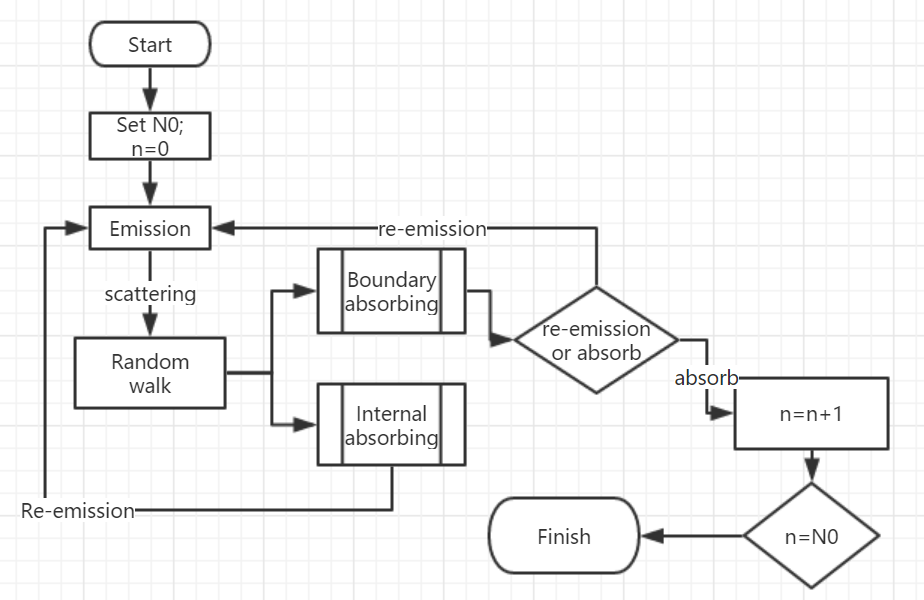
\includegraphics[width=3in]{1.png}
  \caption{Block diagram of the tracing algorithm}
  \label{fig:1}  
\end{figure}


\subsection{Monte Carlo simulation steps}
\subsubsection{Problem formation}
The Two dimensional thermal transport in silicon films with internal heating can be characterized by the two dimensional BTE, $\partial f / \partial t + V_{gx}\partial f / \partial x + V_{gy}\partial f / \partial y = (f_0 - f)/ \tau + \dot{S}_{\Omega}$. 


\begin{figure}[!hbt]
  \centering
  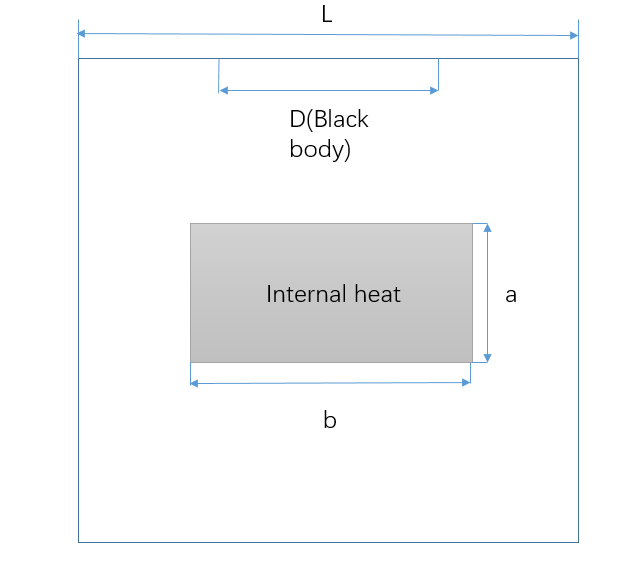
\includegraphics[width=2.5in]{5.png}
  \caption{Two dimensional thermal transport in silicon films with internal heating}
  \label{fig:2}  
\end{figure}

The schematic of simulating object is illustrated in Fig \ref{fig:2}.The upper boundary with the length of D is considered as phonon blackbody, that is to say, phonon are completely absorbed there, which means heat will only conduct to outer space there, while all the other boundaries are adiabatic and the phonon-boundary scattering at them is assumed to be completely diffusive.The internal heat source is implemented by setting the phonon source inside the nanofilms, which is clearly shown in the Fig, and phonons with definite energy will originate within the zone.Then, all the phonon bundles will be traced until they exit through the black-body boundary. \\
\indent The temperature profile then can be obtained from the phonon distribution calculated by our MC simulation\cite{hua1}. More importantly, we should note that since our system is comparable with the phonon MFP, the local thermodynamic equilibrium cannot be established, and the temperature is more a parameter than its conventional meaning of representing a thermal equilibrium state.\\
\indent One famous theory proposed that in that case, the temperature calculated is actually a representation of the average energy of all phonons around a local point\cite{Super}. And we will adopt that explanation and will give our temperature profile according to that.
\subsubsection{Monte Carlo simulation}
The MC technique simulates phonon transport process by random number samplings, equivalent to directly solving the phonon BTE. The phonon tracing algorithm is as follows:
\begin{enumerate}
\item Draw the initial properties(by randomly choose a point in heat source zone) ,for example, $r_0$ of phonon bundle.
\item Calculate the traveling length using the Eq(7), and renew the position of the phonon, $r_{new}=r_0+\Delta r$.
\item If a phonon collides with a boundary, if it is the black-body boundary, set n=n+1(n denotes the number of phonons which emit),or at the adiabatic boundary then
 set the position value at the boundary and let the phonon re-emit from the boundary.
 \item If a phonon does not collide with the boundaries, the phonons just re-emit at $r_{new}$, and we set $r_0=r_{new}$.
 \item Record the frequency phonons get absorbed at each control body(each grid) and when n equals $N_p$($N_p$ is the number of the phonon bundles we trace in simulation), the whole process is finished.
\end{enumerate}
Just one thing should be noticed, although we choose a large number of phonon bundles, we trace only one at a time. When a phonon exits at the black-body boundary, we emit another and repeat till all the phonon bundles has been traced and recorded.

\section{Results}

%\section{Results and Discussions}
\subsection{Results and discussion}

\begin{figure}
\begin{minipage}[t]{0.33\linewidth}
\centering
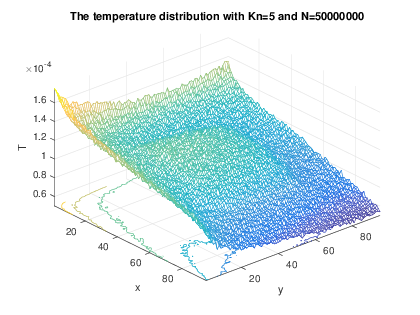
\includegraphics[width=2.2in]{2.png}
\caption{Kn=0.05}
\label{fig:3}
\end{minipage}%
\begin{minipage}[t]{0.33\linewidth}
\centering
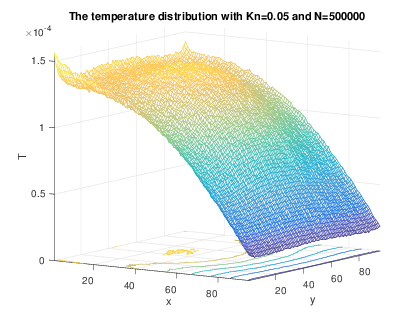
\includegraphics[width=2.2in]{3.png}
\caption{Kn=0.5}
\label{fig:4}
\end{minipage}
\begin{minipage}[t]{0.33\linewidth}
\centering
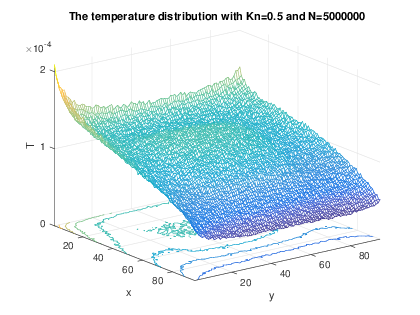
\includegraphics[width=2.2in]{4.png}
\caption{Kn=5}
\label{fig:5}
\end{minipage}%
\end{figure}

\begin{figure}
\begin{minipage}[t]{0.5\linewidth}
\centering
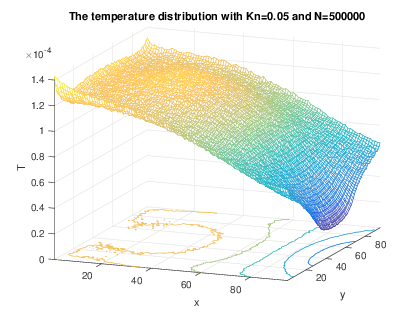
\includegraphics[width=2.2in]{6.png}
\caption{Kn=0.05}
\label{fig:6}
\end{minipage}%
\begin{minipage}[t]{0.5\linewidth}
\centering
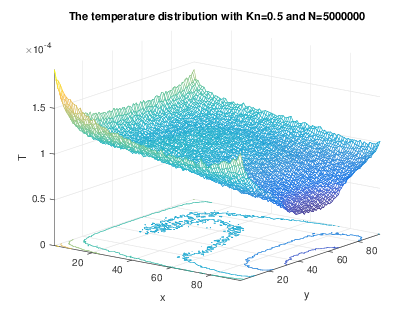
\includegraphics[width=2.2in]{7.png}
\caption{Kn=0.5}
\label{fig:7}
\end{minipage}
\end{figure}

The dimensionless temperature profiles in Si nanofilms are shown in Fig \ref{fig:3},Fig \ref{fig:4},Fig \ref{fig:5}.As Kn = 0, the phonon transport is purely diffusive and the corresponding temperature profile can be calculated by the classical   law. With the increase of the Knudsen number, phonon ballistic transport becomes stronger.
The temperature jumps occur at the boundaries and the temperature
gradient becomes smaller.And we can find there exits a temperature jump between at the boundaries and increase with the Knudsen number.\\
\indent We can conclude that when the kn gets closer to $\infty$, there will be no temperature gradient in the nanofilm and will result a highest temperature jump on the boundaries.\\
\indent And we can know when the kn Number becomes bigger, the scattering decreases and thus it gets harder to reach the equilibrium, so we increase the sampling number from 50,0000 to 5000,0000 as the kn ranges from 0.05 to 5.\\
\indent One thing should be added is the perturbation at the boundary is mainly caused by the truncation error of the computer and we just give up some units to correct and that won't affect the whole temperature profile.




\subsubsection*{Boundary condition changes}
If we narrow the width that the phonons can pass,which are shown in Fig \ref{fig:6} and Fig \ref{fig:7} namely the black-body boundary, we can find the temperature profile will change and the temperature around the exit will be lower. That calculation means this method can be applied to more complex boundary conditions.\\

\subsection{Conclusion}
\begin{itemize}
\item Based on Hua's work on one-dimension study on conductivity which is focuses on the mechanism in the ballistic-diffusive transport, we develop this method to two-dimension and in the future to real devices by considering more complicated boundary conditions and influence.
\item The MC technique can help solve the BTE and gives a valid temperature profile in different Knudsen numbers which is the same with different MFPs in reality. And this will help us understand the heat conduction in nano-films and then develop the optimization.
\end{itemize}

\subsubsection*{Frequency-dependent MC Simulation}
Because we adopt the Gray-body approximation in our MC simulation, we don't consider the phonon frequency effect. However, it is found that, in the room temperature and the region we mainly care about, this a good for calculating the temperature profile. So in next chapter, we will focus a more crucial and interesting , also not fully covered aspect, the phonon properties in interfaces, which also plays a significant role in our goal of tuning the thermal conduction in nano devices.But we still 
summarize the main points of the frequency-dependent MC simulation in Appendix2.





\clearpage

% \footnote{My footnote goes blah blah blah! \dots}


